% !TEX encoding = UTF-8 Unicode

\documentclass[a4paper]{article}

\usepackage{color}
\usepackage{url}
\usepackage[T2A]{fontenc} 
\usepackage[utf8]{inputenc}
\usepackage{graphicx}

\usepackage[english,serbian]{babel}
\usepackage[unicode]{hyperref}
\hypersetup{colorlinks,citecolor=green,filecolor=green,linkcolor=blue,urlcolor=blue}

\begin{document}

\title{Kriptovalute\\ \small{Seminarski rad u okviru kursa\\Računarstvo i društvo\\ Matematički fakultet}}

\author{Petar Rondović\\ mi17167@alas.matf.bg.ac.rs}
\date{14.~septembar 2022.}
\maketitle

\abstract{
Ovaj rad se bavi temom kriptovalute. Prolazi kroz tehnologije i tehnike na kojima je baziran ceo sistem kriptovaluta i ukazuje u koje još svrhe se može upotrebiti. Ukratko se spominju osnovni koncepti razvoja novca i 
navodi se nekoliko primera kriptovaluta i njihove karakteristike.
\tableofcontents

\newpage

\section{Uvod}
\label{sec:uvod}
Kriptovalute su tip valute koje postoje digitalno i koriste kriptografiju za zaštitu transakcija. One nemaju centralni organ za izdavanje ni za regulisanje nego umesto toga koriste decentralizovani sistem za zapisivanje transakcija i izdavanje novih jedinica kriptovalute \cite{kriptovalute1}. Prva kriptovaluta, Bitcoin, nastala je 2009. za vreme najhaotičnijeg perioda u istoriji SAD-a. Za vreme globalne finansijske krize od 2007. do 2009. nepoverenje u banke i centralne vlade bilo je na vrhuncu. Ima smisla da se decentralizovani sistem za plaćanje pojavi u ovakvom periodu \cite{istorijabitcoina}.


\section{Kratak uvod o istoriji novca}
\label{sec:istorija}
U početku, jedini oblik kupovine je bila trampa. Trampa je direktna razmena usluga i sredstava, kao primer zamisliti farmera koji se dogovara sa obućarem, za koju količinu pšenice može dobiti par cipela. Problem nastaje ako niko neće da prihvati ponudu. Razlog može biti ili ne slaganje o vrednosti u ponudi, ili nema potrebe za stvar koja se nudi.

Polako kroz vekove nastaje valuta u obliku često razmenjivanih stvari, kao što su krzna, so i oružija. One su predstavljale sredstva razmene, čiji je najveći uspeh u skraćivanju vremena celog procesa trampe. Nova sredstva razmene postaju novčići pravljenji od plemenitih metala, okarakterisani malom veličinom i inherentnoj vrednosti.

Eventualno banke počinju da koriste papirne novčanice za svoje klijente umesto metalnih novčića.  One su mogle da se odnesu u banku i zamene za njihovu nominalnu vrednost u obliku novčića, najčesće napravljenih od zlata ili srebra. Ovakav oblik novca mogao je da se koristi za razmenu usluga i sredstava. Funkcionisalo je isto kao i u modernom svetu, jedina razlika je što su ih izdavale banke i privatne institucije, a ne državna uprava kao sto je to slučaj danas \cite{istorijanovca}.

Razvojem tehnologije, pronađeni su jos praktičniji načini da se razmenjuju stavri. Sve više ljudi kupuje preko interneta i koristi kartice za plaćanje. U ovoj fazi više nema direktnog kontakta sa novcem. Nema više novčića, novčanica niti razmene, sve su samo vrednsoti u tabeli. Kada se nešto kupi preko interneta, sve se svodi na to da banka kupca ažurira njegov račun, što se takođe dešava sa računom vezanim za prodaju.

Kriptovalute u praksi funkcionišu na isti način.

\section{Kriptovalute}
\label{sec:kriptovalute}
Kriptovaluta je digitalni sistem za plaćanje koji ne zavisi od banaka za verifikovanje transakcija. On je baziran na P2P (eng. peer to peer) sistemu koji omogućava da bilo ko, bilo gde prima ili šalje uplate. Umesto nošenja pravog novca i njegovog korišćenja u stvarnom svetu, naplaćivanja kriptovalutama postoje samo kao digitalni zapisi u onlajn bazi podataka opisivajući određene transakcije. Transakcije koje se izvršavaju kriptovalutom, zapisuju se u javnu glavnu knjigu (eng. ledger). Kriptovalute se čuvaju i digitalnim novčanicima.
Naziv je dobila zato što koristi enkripciju za verifikovanje podataka. To znači da se napredno kodiranje koristi za čuvanje i razmenu kriptovaluta u novčanicima i u glavnoj knjizi. Cilj enkripcije je da zagarantuje sigurnost \cite{kriptovalute1}.

\newpage

\section{Blockchain}
\label{sec:blockchain}
Blockchain je otvorena i podeljena knjiga koja zapisuje sve transakcije u obliku koda. U praksi je kao zapisnik distribuiran između mnogo računara širom sveta. Transakcije su zapisane u "blokovima" koje se nalaze u "lancu" predhodnih transakcija kriptovaluta. Zamisliti knjigu u kojoj zapisujemo sve na šta smo potrošili pare. U ovom primeru bi stranice bile blokovi, a cela knjiga bi predstavljala lanac.

Sa blockchain-om, svako ko koristi kriptovalute ima svoju kopiju knjige kako bi se osnovao ujedinjen zapisnik transakcija. Pri svakoj novoj transakciji, ažuriraju se sve kopije blockchain-a, održavajući tačnost.\cite{kriptovalute2} Ovaj koncept je predložen kao istrživački projekat 1991. da bi se 2009. iskoristio za Bitcoin i u sledećim godinama znatno proširio sa porastom različitih kriptovaluta \cite{blockchain}.


\subsection{Decentralizacija i transparentnost}
\label{subsec:decentralizacija}
Blockchain funkcioniše tako što podatke sačuvane u bazi podataka deli između više čvorova mreže na različitim lokacijama. Prednost ovakvog sistema je što nije sve na jednom mestu, pa ako dođe do nestanka struje, prekida interneta ili nekih zlonamernih aktivnosti, neće biti gubitka podataka. Zbog većeg broja kopija, ako neko promeni podatke u jednoj instanci baze podataka, ostale kopije će sprečiti promenu. Ako su promene samo na jednom čvoru, proverom ostalih čvorova će se odrediti čvor koji ima netačne podatke. Kako bi to izgledalo se može videti na slici \ref{fig:proverakopija}.

\begin{figure}[h!]
\begin{center}
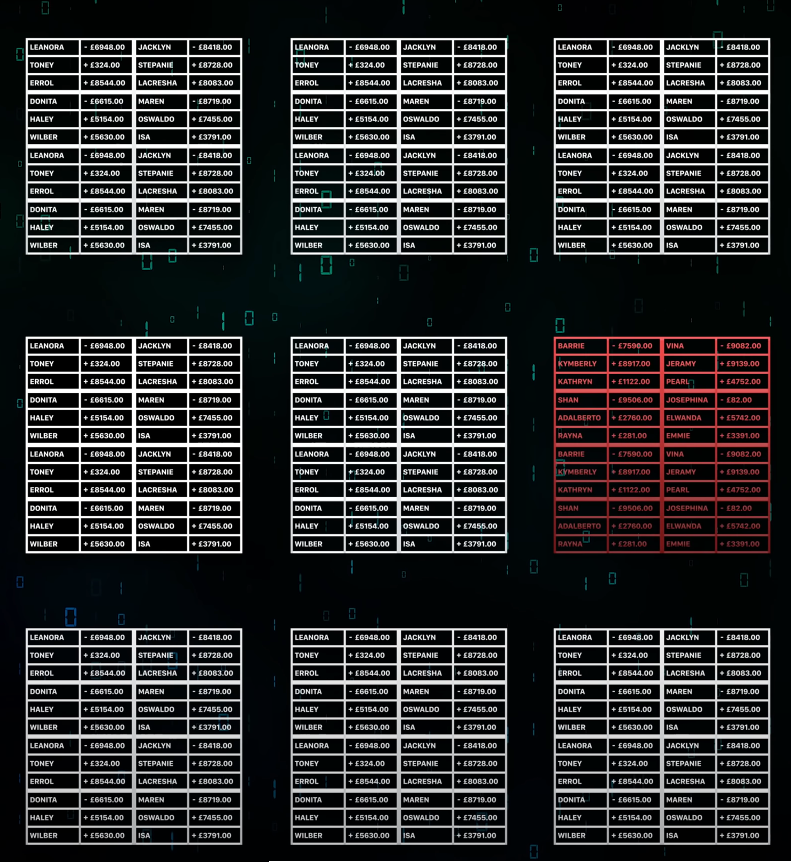
\includegraphics[scale=0.4]{slike/slika1.png}
\end{center}
\caption{Predstavaljanje provere čvorova kada postoji kopija koja se ne poklapa}
\label{fig:proverakopija}
\end{figure}

\newpage

U ovakvom sistemu nije moguće promeniti podatke cele mreže menjanjem samo jednog njenog čvora. Takođe se omogućava očuvanje informacija i istorije podataka. Takav zapisnik sadrži listu transakcija, ako su u pitanju kriptovalute, ali blockchain može sadržati i druge informacije, kao što su ugovori, indentifikacije ili inventar proizvoda kompanije.

Zbog decentralizovane prirode blockchain-a, sve transakcije se mogu videti u okviru svoje kopije ili korišćenjem blockchain pretraživača koji omogućavaju praćenje transakcija uživo. Svaki čvor ima svoju kopiju lanca koja se ažurira dodavanjem novih blokova. Ovo omogućava praćenje korišćenja kriptovalute. Ima slučajeva gde su razmene bile hakovane. Haker jeste ostao anoniman, ali je moguće pratiti korišćenje ukradene kriptovalute. Naravno, imformacije u blockchain-u su enkriptovane i samo vlasnik zapisnika može da dekriptuje podatke. Tako se održava anonimnost i transparentnost \cite{blockchain}.


\subsection{Sigurnost}
\label{subsec:sigurnost}
Blockchain održava dectentralizovanu sigurnost i poverenje na više načina. Za početak, blokovi se čuvaju linearno i hronološki, odnosno dodaju se na kraj lanca. To otežava vraćanje kroz lanac jer bi se promenile informacije u bloku, osim ako većina mreže to ne odobri. Svaki blok sadrži svoj heš, kao i heš bloka pre njega,
slika \ref{fig:blockchain}. Heš se pravi od podataka u okviru bloka, pa ako dođe do promene neke informacije, promeniće se i heš.

\begin{figure}[h!]
\begin{center}
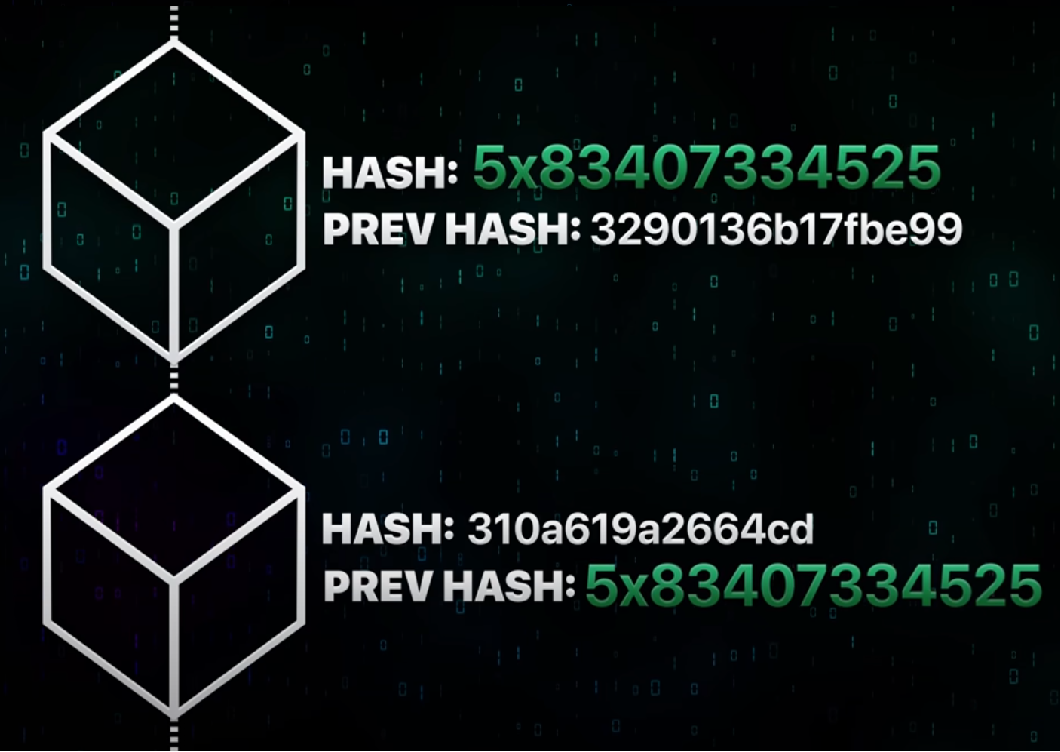
\includegraphics[scale=0.25]{slike/slika2.png}
\end{center}
\caption{Blockchain}
\label{fig:blockchain}
\end{figure}


Ako haker, koji takođe ima čvor u mreži blockchain-a, želi da promeni podatke i ukrade kriptovalutu od drugih, nije dovoljno da promeni samo svoju kopiju. Poređenjem sa ostalim kopijama će se primetiti odstupanje i ta kopija će se smatratiti nelegitimnom. Za uspešno hakovanje, potrebno je promeniti više od 50\% kopija. Takav napad bi zahtevao puno novca i sredstava jer bi morali promeniti svaki blok u lancu koji zbog promene imaju i promenjen heš \cite{blockchain}.

\newpage

\subsection{Blockchain kao tehnologija}
\label{subsec:tehnologija}
Stuart Haber i W. Scott Stornetta su istraživači koji su 1991. izmislili koncept blockchain-a. Hteli su da implementiraju sistem u kome nije moguće menjati vremena dokumenata. Prošle su skoro dve decenije dok blockchain nije dobio svoju upotrebu u stvarnom svetu sa pokretanjem Bitcoin-a 2009. Ključnu stvar koju treba razumeti je da se blockchain u kriptovalutama koristi samo kao transparentni zapisnik plačanja, ali u teoriji  se može koristiti za nepromenljivo zapisivanje bilo kog broja imformacija. Može biti u obliku transakcija, kao što je već diskutovano, glasova za vreme izbora, inventara proizvoda, indentifikatora i mnogih drugih.

Trenutno postoji mnogo projekata koji pokušavaju da implementiraju blockchain sisteme kako bi pomogli društvu. Jedan primer je osigurano glasanje na demokratskim izborima. Karakteristika nepromenljivosti podataka znatno otežava pokušaje lažnog glasanja. Sistem bi funkcionisao tako što bi svaki građanin dobio token. Kandidati bi imali svoje adrese novčanika i glasači bi slali svoje tokene na adresu kandidata za kojeg žele da glasaju. Karakteristike transparentnosti bi eliminisali potrebu za brojanjem glasova i mogućnosti praćenja tokena bi sprečile manipulisanje glasovima \cite{blockchain}.


\section{Tehnike verifikacije}
\label{sec:verifikacija}
Za sprečavanje prevara, nad transakcijama se primenjuje jedna od dve tehnike validacije, proof of work ili proof of stake \cite{kriptovalute2}.

\subsection{Proof of work}
\label{subsec:work}
Proof of work je tehinka verifikacije gde algoritam generiše problem za koji se računari trkaju da ga reše.
Miner je naziv koji je pripisan svakom računaru koji učestvuje u rešavanju matematičkog problema koji pomaže pri verifikaciji grupe transakcija, koje predstavaljaju blok, i dodaje ih u blockchain. Prvi računar koji to uspešno uradi biva nagrađen malom količinom odgovarajuće kriptovalute.
Trka za rešavanje problema zahteva veliku snagu računara i potrošnju energije. To znači da miner-i jedva zarade nešto za validaciju transakcija kada uzmemo u obzir potrošnju struje i cenu samog računara \cite{kriptovalute2}.

\subsection{Proof of stake}
\label{subsec:stake}
Neke kriptovalute koriste proof of stake kao tehinku validacije da bi smanjili potrošnju energije potrebnu za proveru transakcija. Ovom tehnikom, broj transakcija koje korisnik može da odobri zavisi od količine kriptovalute koju je spreman da uloži, ili na neko vreme zaključa u komunalni sef, da bi imao šansu da učestvuje u procesu validacije.
Svako ko uloži kriptovalutu ima šansu da bude izabran za validaciju transakcije, ali šansa da neko bude izabran sa povećavaju sa većim ulogom.
Zato što proof of stake ne zahteva intenzivna izračunavanja koja zahtevaju veliku količinu energije, znatno je efikasnije od proof of work i omogućava brza izvršavanja verifikacija ili potvrda transakcija.
Kao primer, prosečno vreme potrebno za transakciju kod Bitcoin-a je u proseku najmanje 10 minuta, dok u poređenju Solana, kripto platforma koja koristi proof of stake, izvršava u proseku 3000 transakcija po sekundi.
Takodje, Ethereum, Bitcoin-ov najveći konkurent, u potpunosti prelazi na proof of stake sistem \cite{kriptovalute2}.

Obe tehnike validacije se zasnivaju na mehanizmima konsenzusa. To znači da iako obe tehnike koriste pojedince za validaciju transakcije, one moraju biti proverene i odobrene od strane većine vlasnika kopija glavne knjige.\cite{kriptovalute2}


\section{Različite kriptovalute}
\label{sec:različitekriptovalute}

\subsection{Bitcoin}
\label{subsec:bitcoin}
Bitcoin je prva i ubedljivo najpopularnija kriptovaluta. Osnovan je 2009. od strane čoveka ili grupe pod pseudonimom Satoshi Nakamoto. Dizajniran je da bude nezavisan od državne uprave ili centralne banke. Zavisi od blockchain sistema i kao tehniku verifikacije koristi proof of work. Popularnost Bitcoin-a je tolika da je ogromno korišćenje energije, koje održavanje sistema zahteva, dovela u pitanje brigu o zagađenju životne sredine \cite{različitekriptovalute}.

\begin{figure}[h!]
\begin{center}
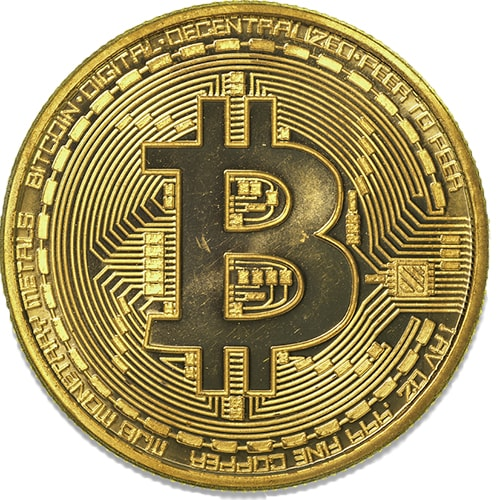
\includegraphics[scale=0.3]{slike/slika3.jpg}
\end{center}
\caption{Bitcoin logo}
\label{fig:bitcoin}
\end{figure}


\subsection{Ethereum}
\label{subsec:ethereum}
Kao Bitcoin, Ethereum je baziran na blockchain tehnologiji. Za razliku od Bitcoin-a, dizajniran je kao programabilni blockchain odnosno nije napravljen da podrži samo valutu, nego najpre da omogući korisnicima mreže da prave, objavljuju i monetizuju decentralizovane aplikacije. Ether, izvorna valuta Ethereum-a, napravljena je kao oblik plaćanja u okviru platforme. Ether možemo posmatrati kao gorivo koje pokreće Ethereum blockchain. Ethereum je blockchain na kom je došlo do ogromnog zainteresovanja za NFT o čemu će biti više priče u sledećem poglavlju.

Kao dva najpopularnija predstavnika, mnogo ljudi direktno poredi Bitcoin i Ethereum iako su napravljeni u dve različite svrhe. Bitcoin je mreža za digitalni novac koja olakšava transakcije bez potrebe za centralnim autoritetom, dok Ethereum, često nazivan računar sveta, baziran na tehnologiji Bitcoin-a dodaje još i pametne ugovore (eng. smart contracts). Oni omogućavaju pravljenje decentralizovanih aplikacija koje obuhvataju širok spektar programa. Ethereum takođe koristi proof of work kao sistem za validaciju, ali kao što je već navedeno, planiraju da pređu na proof of stake sistem. Još jedna razlika je što je Bitcoin ograničen na 21 milion jedinica Bitcoin tokena, dok je Ether neograničen \cite{različitekriptovalute}.


\begin{figure}[h!]
\begin{center}
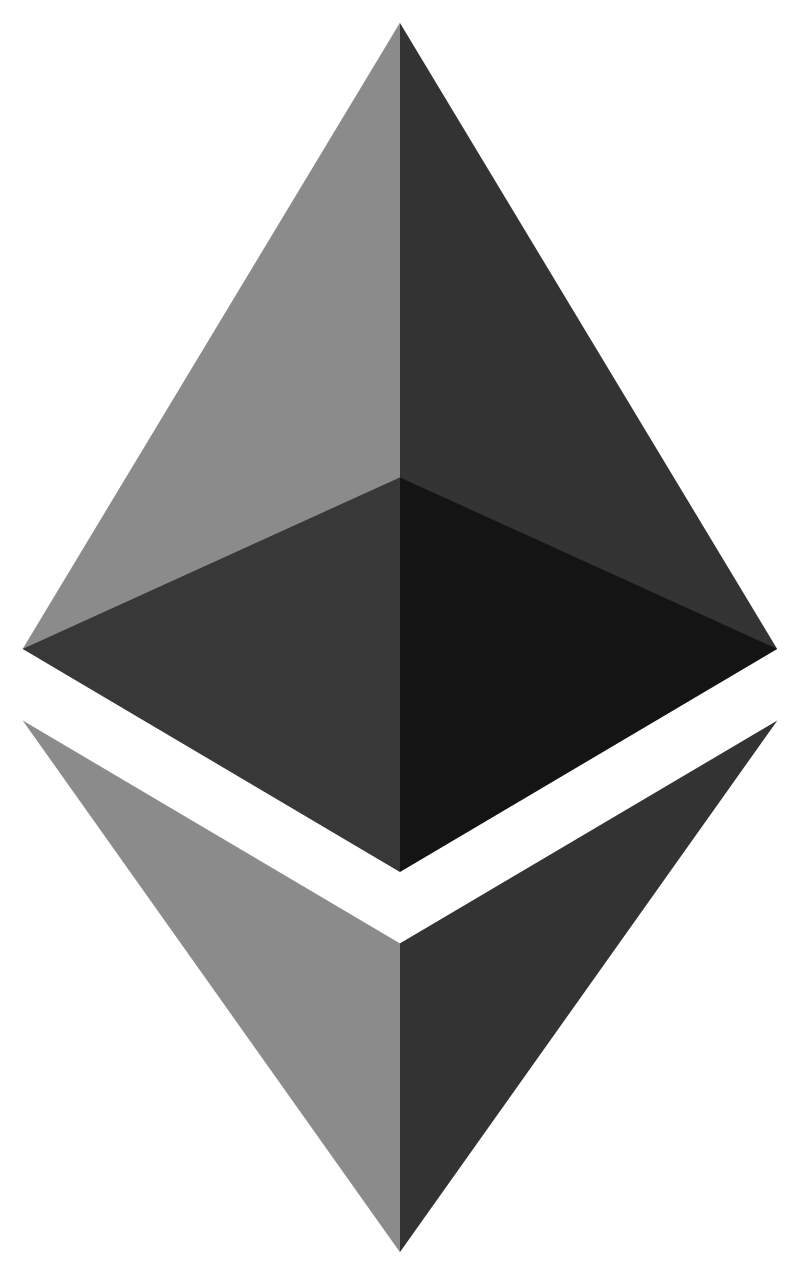
\includegraphics[scale=0.1]{slike/slika4.png}
\end{center}
\caption{Ethereum logo}
\label{fig:ethereum}
\end{figure}


\subsection{Cardano}
\label{subsec:cardano}
Cardano je blockchain platforma sa proof of stake sistemom verifikacije koja ima funkcionalnosti pametnih ugovora. Cardano je poznat po svom fokusu na akademska istraživanja, velikoj propusnosti transakcija u sekundi i energetski efikasnom konsenzus mehanizmu Ouroboros. ADA je izvorna valuta Cardano mreže i služi da olakša transakcije i izvršavanje pametnih ugovora.  Ada Lovelace, matematičarka 19. veka, je inspiracija za naziv valute. Cardano se razvija u pet faza ka postizanju cilja razvijanja mreže u platformu decentralizovanih aplikacija. Svaka faza u planu zasnovana je na istraživačkim okvirima i recenziranim uvidima koji su pomogli za uspostavljanje akademske reputacije.\cite{različitekriptovalute}

\begin{figure}[h!]
\begin{center}
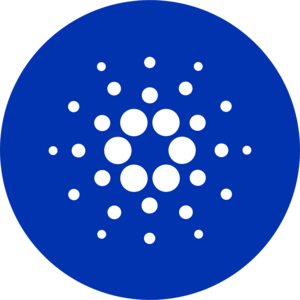
\includegraphics[scale=0.4]{slike/slika5.png}
\end{center}
\caption{Cardano logo}
\label{fig:cardano} 
\end{figure}


\newpage

\section{Non-fungible token (NFT)}
\label{sec:nft}
\textbf{Zamenljivost (eng. Fungibility)} znači da je nešto moguće zameniti nečim indentičnim. Kada je nešto zamenljivo, tipično ih je mnogo istih. Zamenljiv token se može podeliti i zemeniti za neki drugi.

\textbf{Nezamenljivost (eng. Non-fungibility)} nudi jedinstvenost kao glavni atribut. Nezamenljiv token je jedinstven i ne može postojati još jedan isti. Kao primer, avionska karta je jedinstvena, odnosi se na određeno mesto, određeni let u određeno vreme.

Nezamenljiv token (eng. NFT) je tip kriptografskog tokena koji predstavlja jedinstvenu stvar. Te stvari mogu biti digitalne ili fizičke. Nezamenljivi tokeni omogućavaju vlasnicima da dokažu vlasništvo i autentičnost neke stvari. Takođe olakšava proces kupovine preduzećima ili pojedincima jer mogu da veruju da će dobiti ono što su kupili zbog provere identifikatora nezamenljivog tokena te stvari \cite{nft}. Karakteristike nezamenljivih tokena:\\ 

\textbf{Nedeljivost:} Oni se ne mogu podeliti kada je u pitanju njihova funkcionalnost. Avionska karte se ne može iskoristit nekim njenim delom već samo u celosti, jer se odnosi samo na jedno mesto koje samo jedna osoba može da iskoristi.\\ 

\textbf{Retkost:} Nedeljivi tokeni mogu biti retki i to je nešto što im daje vrednost. Iako je moguće generisati mnogo sredstava, tako je isto moguće limitirati broj tokena.\\

\textbf{Jedinstvenost:} Jedinstveni su jer ne postoje dva ista nezamenljiva tokena. Metapodaci nezamenljivih tokena su nepromenljivi zapisi koji im daju sertifikate autentičnosti.\\

\textbf{Vlasništvo:} Žive u blockchain-u u okviru nečijeg računa. Kreatori nezamenljivog tokena kontrolišu privatni ključ računa u kom se nalazi i imaju slobodu da ga transferuju na nečiji račun.\\

\textbf{Transparentnost:} Zbog karakteristika blockchain-a gde zapisi izdavanja, transfera i aktivnosti nekog tokena mogu biti javno verifikovani, kupci mogu da veruju i verifikuju autentičnost nekog željenog tokena.\\

\textbf{Kompatibilnost:} Nezameljivi tokeni se mogu zameniti, kupiti ili prodati preko različitih blockchain sistema, koristeći decentralizovani most ili centralizovane službe.


\newpage


\section{Zaključak}
\label{sec:zaključak}
Iako kriptovalute imaju mnogo prednosti, kao što su brza internacionalna plaćanja bez brige o kursevima valute i bez ograničenja, nisu ni one savršene. Ako bi se u potpunosti prešlo na sistem kriptovaluta, najveći izazov predstavlja određivanje poreza koji je bitan za razne aspekte funkcionisanja države. Problem je još što iako je blockchain siguran sistem, moguće je izvršiti hakerske napade na digitalne novčanike koji nisu deo sistema. Ali najveći problem predstavlja određivanje vrednosti.

Nepostoji ništa na osnovu čega bi se odredila tačna vrednost kriptovalute, sve su samo spekulacije. Vrednost se trenutno određuje time koliki je nivo zainteresovanosti ljudi i koliko su spremni da ulože. Za uspešno ulaganje je potrebno veliko razumevanje samog sistema i ekonomije, što prosečan stanovnik nema, a zbog velike popularnosti može da se uključi u celu priču i potencijalno sebi napravi štetu. Zbog trenutne krize i situacije u svetu, vrednost kriptovaluta je opala na najniži nivo posle dugog perioda uzastopnog rasta.

Ono što jeste bitno je tehnologija na kojoj je sve bazirano. Internet je primer tehnologije koji se drastično promenila u poređenju na prve oblike i koji nastavlja da se razvija. Blockchain ima dobre karakteristike koje su privukle veliku pažnju. Tako da iako sada nisu prisutni svuda, mogu postati deo svakodnenog života i to u nekom potupno drugom obliku.

\addcontentsline{toc}{section}{Literatura}
\appendix

\iffalse
\bibliography{literatura} 
\bibliographystyle{plain}
\fi

\begin{thebibliography}{9}

\bibitem{kriptovalute1}
\href{https://www.kaspersky.com/resource-center/definitions/what-is-cryptocurrency}{What is cryptocurrency and how does it work?}

\bibitem{istorijabitcoina}
\href{https://money.usnews.com/investing/articles/the-history-of-bitcoin}{The History of Bitcoin, the First Cryptocurrency}

\bibitem{istorijanovca}
\href{https://www.investopedia.com/articles/07/roots_of_money.asp}{The History of Money}

\bibitem{kriptovalute2}
\href{https://www.forbes.com/advisor/investing/cryptocurrency/what-is-cryptocurrency/}{What Is Cryptocurrency?}

\bibitem{blockchain}
\href{https://www.investopedia.com/terms/b/blockchain.asp}{Blockchain Facts: What Is It, How It Works, and How It Can Be Used}

\bibitem{različitekriptovalute}
\href{https://www.sofi.com/learn/content/understanding-the-different-types-of-cryptocurrency/}{Understanding the Different Types of Cryptocurrency}

\bibitem{nft}
\href{https://hedera.com/learning/tokens/what-is-a-non-fungible-token-nft?adgroupid=139332525739&utm_term=&utm_campaign=hh19c1&utm_source=sem&utm_medium=ppc&utm_content=611328684444&hsa_acc=1782665900&hsa_cam=1717906681&hsa_grp=139332525739&hsa_ad=611328684444&hsa_src=g&hsa_tgt=dsa-1692334474972&hsa_kw=&hsa_mt=&hsa_net=adwords&hsa_ver=3&gclid=EAIaIQobChMIkarYjMSS-gIVkAwGAB2K9gOcEAAYAyAAEgJqcPD_BwE}{What is a non-fungible token (NFT)?}





\end{thebibliography}


















\end{document}